\documentclass[../portafolio.tex]{subfiles}

% Solo agregue paquetes en el preámbulo de ../portafolio.tex

\begin{document}

% En esta sección, explique en detalle los siguientes aspectos:
% - Fecha de realización de la actividad
% - Título de la actividad (dentro de \section)
% - Un párrafo explicando cuál es el objetivo de la actividad
% - Nombre de personas con quien trabajó en la actividad
% - Una selección de evidencias de que usted hizo esta actividad (imágenes, códigos, respuestas a un problema teórico, etc.)
% - Una conclusión breve (qué aprendió con la actividad, qué no entendió, qué faltó trabajar, qué recomienda para futuras sesiones)

% Numero máximo de palabras en esta sección: 1000 palabras.

%%%%%%%%%%%%%%%%%%%%%%%%%%%%%%%%%%%%%%%%%%%%%%%%%%%%%%%%%%%%%%%%%%%%%%%%%%%%%%%%
\section{Resoluci\'on Numerica de Ecuaciones Diferenciales Ordinarias}   % ejemplo: Derivadas numéricas , introducción a git , 

\hfill \textbf{Fecha de la actividad:} 23 de septiembre de 2022

\medskip

%---------------------------------------------------------------------------------
% Introducción/objetivos de la actividad
Durante esta actividad se ense\~n\'o los m\'etodos computacionales para poder encontrar las soluciones de ecuaciones diferenciales ordinarias ocupando dos m\'etodos, el m\'etodo de Euler y el m\'etodo de Euler-Cromer. Lo interesante de resolver ecuaciones diferenciales ordianrias de manera computacional es que el output (resultado) de nuestro codigo no es explicitamente una funci\'on, sino, una colecci\'on de puntos. En la parte de laboratorio nos enfocamos mayoritariamente en el m\'etodo de Euler.

%---------------------------------------------------------------------------------
% Con quién hizo esta actividad
Esta actividad la realic\'e con Mart\'in Sepulveda
%---------------------------------------------------------------------------------
% Selección de evidencias
	\subsection{Ejercicio 1}
		Para la resoluci\'on de este primer ejercicio debemos reescribir las ecuaciones de Lotka-Volterra, las cuales son: 
			
			\begin{align}				
				\frac{dP}{dt} &= \alpha P - \beta PD  \label{eq:lotvol1} \\
				\frac{dD}{dt} &= - \gamma D + \delta PD \label{eq:lotvol2}
			\end{align} 

Con el objetivo de poder reescribir la segunda ecuaci\'on de Lotka-Volterra lo que haremos es:
	\begin{align*}
		\frac{dD}{dt} \frac{1}{\gamma} &= -D + \Pi D \\
		\frac{dD}{dt} \frac{1}{\gamma} &= D(\Pi -1)
	\end{align*}
Luego tomando $ D = \Delta \frac{\alpha}{\beta}$ tendremos:

	\begin{align*}
		\frac{d}{dt}\left[ \frac{\Delta \alpha}{\beta} \right] &= \Delta \frac{\alpha}{\beta}~(\Pi - 1) \\
		\frac{\alpha}{\beta} ~ \frac{d \Delta}{dt} &= \Delta \frac{\alpha}{\beta} ~(\Pi -1) \\
	\end{align*}
Recordando que $\tau = \alpha t$, reemplazamos en la \'ultima expresi\'on resultando en:
	\begin{align*}
	\frac{d \Delta}{d \tau} &= \frac{1}{\alpha} ~ \Delta ~  (\Pi -1) \\
	\frac{d \Delta}{d \tau} &= \mu \Delta ~ (\Pi -1) \\
	\end{align*}
Donde, en el \'ultimo paso reemplazamos $\frac{1}{\alpha} = \mu$ para poder obtener el resultado mostrado anteriormente. \\
As\'i hemos podido reescribir la segunda ecuaci\'on de Lotka-Volterra. Luego, para poder reescribir la primera ecuaci\'on (\ref{eq:lotvol2}) seguimos un proceso similar resultando en: 
	\begin{align*}
		\frac{d \Pi}{d \tau} = \Pi(1- \Delta)
	\end{align*}
	
Para encontrar la soluci\'on a ecuaci\'on diferencial ordinaria (\ref{eq:lotvol1}) y (\ref{eq:lotvol2}), donde $\Pi (0)$ y $\Delta(0)$ que tiene condiciones inciales, ocupamos el codigo \ref{cod:edoin}.

\begin{listing}
	\begin{pythoncode}
t = np.arange(0, 40, 0.1)
h = 0.1 

pi = np.zeros(len(t))
delta = np.zeros(len(t))

#Condiciones inciales 
mu = 1
pi[0] = 0.1
delta[0] = 5.0

for n in range(len(t)-1):
    pi[n+1] = pi[n] + h*pi[n]*(1-delta[n])
    delta[n+1] = delta[n] + h*mu*delta[n]*(pi[n+1]-1)
    \end{pythoncode}
    \caption{Algoritmo para resolver Ecuaci\'on Diferencial Ordinaria (\ref{eq:lotvol1}) y (\ref{eq:lotvol2}) con valores inciales}
	\label{cod:edoin}
\end{listing}


Luego podemos graficar las ecuaciones (\ref{eq:lotvol1}) y (\ref{eq:lotvol2}) en intervalos especificos, $0 \leq t \leq 40$, y condiciones inciales $\mu = 1, \Pi(0) = 1.0 $ y $\Delta(0) = 5.0$. As\'i, graficando obtenemos el gr\'afico \ref{graph:presa-depre}, el codigo para este grafico se encuentra en \href{run:src/lab04.py}{este archivo}. A partir de este gr\'afico podemos notar la relaci\'on en la poblaci\'on de una especie de presa y su correspondiente depredeador, como el incremento de una genera el incremento tard\'io de la otra y como este \'ultimo crecimiento genera una disminuci\'on en la poblaci\'on de la presa.

\begin{figure}
\centering
	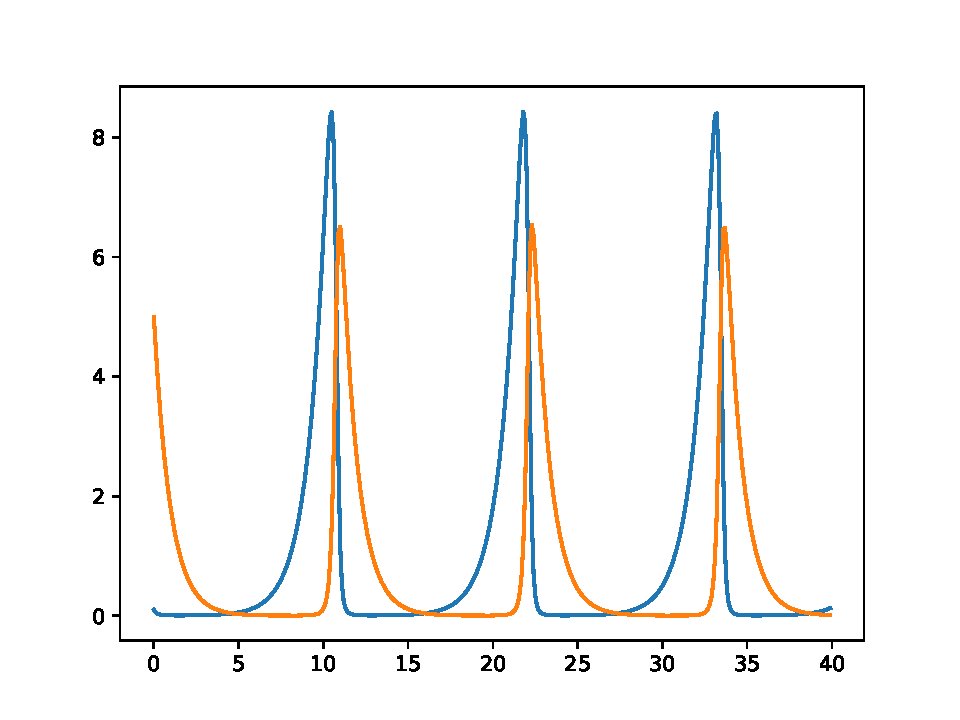
\includegraphics[scale=0.6]{tex/img/presa-depre.pdf}
	\caption{Gr\'afico de las funciones dadas en (\ref{eq:lotvol1}) y (\ref{eq:lotvol2}) en intervalos espec\'ificos.}
	\label{graph:presa-depre}
\end{figure}

Continuando con el laboratorio podemos graficar como se comporta en funci\'on del tiempo (y durante varios ciclos) las poblaci\'ones de una relaci\'on entre la presa y su depredador, esto lo podemos ver en el gr\'afico \ref{graph:chingon}. Este grafico fue realizado con el codigo que se puede encontrar en \href{run:src/graph-chido-edos.py}{este archivo}.

\begin{figure}
\centering
	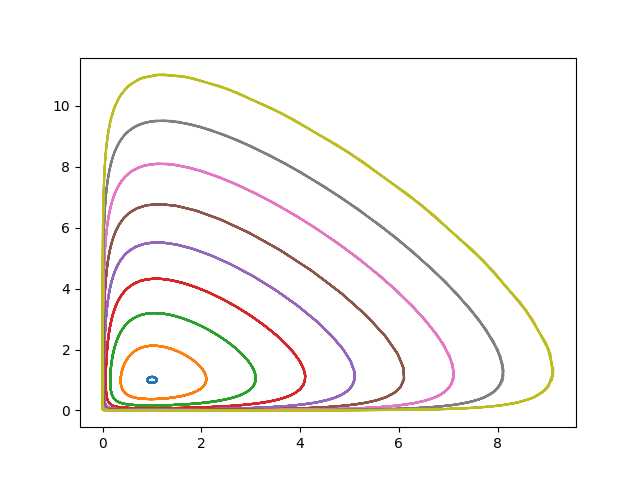
\includegraphics[scale=0.5]{tex/img/graph-chido.png}
	\caption{Grafico espacio de fase en la relaci\'on presa depredador}
	\label{graph:chingon}
\end{figure}

Finalmente, graficamos la constante que las ecuaciones (\ref{eq:lotvol1}) y (\ref{eq:lotvol2}) nos entregan, la cual esta dada por:

\begin{align}
	C = \ln \Delta - \Delta + \mu (\ln \Pi - \Pi) \label{eq:cte}
\end{align}

Ecuaci\'on que vemos en la grafica \ref{eq:cte}. Como podemos ver, se pueden apreciar ciertos peaks en la grafica que nos hacen pensar que no es una constante tan constante como la creemos, sin embargo, en funci\'on que alargamos el intervalo de tiempo esta l\'inea se ir\'a aplanando y tomando la forma de una constante como las solemos conocer.

\begin{figure}
\centering
	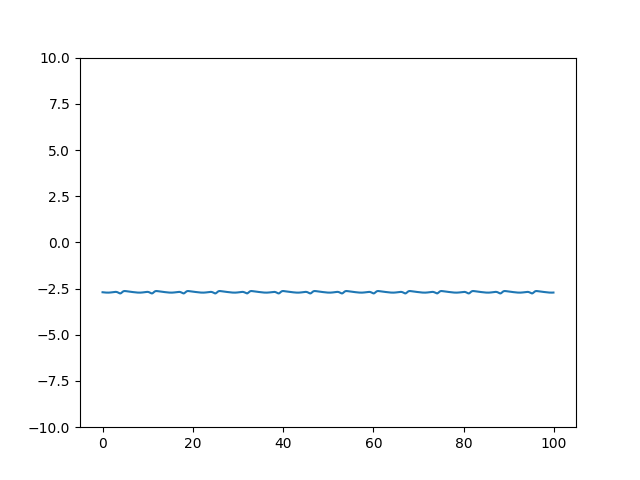
\includegraphics[scale=0.5]{tex/img/cte.png}
	\caption{Grafico de la Constante dada en (\ref{eq:cte}).}
\end{figure}



\end{document} 
